\documentclass[a4paper,20pt]{article}
\usepackage{amsmath,amssymb,epsf,epsfig,times}
\usepackage{multicol}
\usepackage[all]{xy}
\usepackage{color}
\usepackage{ctex}
\usepackage{subfigure}
\usepackage{url,cite}
\usepackage{tikz}
\usepackage[english]{babel}
\usepackage[utf8]{inputenc}

\usepackage{pdfpages}

%\usepackage{caption}
%
%\usepackage[font=small,labelfont=bf,labelsep=none]{caption}
\usepackage[font=default,labelfont=bf,labelsep=period]{caption}

\usepackage{makecell}
\usepackage{booktabs} %引入三线表
\usepackage{diagbox}
\usepackage{multirow}

\usepackage{fancyhdr}
\usepackage{float}
\usepackage{ulem}

\usepackage{listings}
\usepackage{xcolor}

\usepackage{enumerate}
\usepackage{pifont}
\lstset{
    basicstyle          =   \sffamily,          % 基本代码风格
    keywordstyle        =   \bfseries,          % 关键字风格
    commentstyle        =   \rmfamily\itshape,  % 注释的风格,斜体
    stringstyle         =   \ttfamily,  % 字符串风格
    flexiblecolumns,                % 别问为什么,加上这个
    numbers             =   left,   % 行号的位置在左边
    showspaces          =   false,  % 是否显示空格,显示了有点乱,所以不现实了
    numberstyle         =   \zihao{-5}\ttfamily,    % 行号的样式,小五号,tt等宽字体
    showstringspaces    =   false,
    captionpos          =   t,      % 这段代码的名字所呈现的位置,t指的是top上面
    frame               =   lrtb,   % 显示边框
}
\lstdefinestyle{Python}{
    language        =   Python, % 语言选Python
    basicstyle      =   \zihao{-5}\ttfamily,
    numberstyle     =   \zihao{-5}\ttfamily,
    keywordstyle    =   \color{blue},
    keywordstyle    =   [2] \color{teal},
    stringstyle     =   \color{magenta},
    commentstyle    =   \color{red}\ttfamily,
    breaklines      =   true,   % 自动换行,建议不要写太长的行
    columns         =   fixed,  % 如果不加这一句,字间距就不固定,很丑,必须加
    basewidth       =   0.5em,
}

\newtheorem{theorem}{Theorem}[section]
\newtheorem{lemma}{Lemma}[section]
\def\proof{\noindent{\it Proof: }}
\def\QED{\mbox{\rule[0pt]{1.5ex}{1.5ex}}}
\def\endproof{\hspace*{\fill}~\QED\par\endtrivlist\unskip}
\newcommand{\re}{\mathbb{R}}
\def\sV{\mathcal{V}}
\def\sS{\mathcal{S}}
\def\sQ{\mathcal{Q}}

\newcommand{\mc}{\mbox{: }}

\newcommand{\normsq}[1]{\left\|#1\right\|^2}
\newcommand{\norm}[1]{\left\|#1\right\|}
%\newcommand{\sgn}[1]{\mbox{sgn}(#1)}
\newcommand{\pde}[2]{\frac{\partial #1}{\partial #2}}
\newcommand{\fundef}[3]{#1:#2\to #3}
\newcommand{\abs}[1]{\left|#1\right|}
\newcommand{\mymatrix}[2]{\left(\begin{array}{#1}#2\end{array}\right)}
\newcommand{\defeq}{\stackrel{\triangle}{=}}
\newcommand{\paren}[1]{\left(#1\right)}
%\theoremstyle{plain} \newtheorem{theorem}{Theorem}
%\theoremstyle{plain} \newtheorem{algorithm}{Algorithm}
\newtheorem{axiom}[theorem]{Axiom}
\newtheorem{definition}[theorem]{Definition}
\newtheorem{assumption}[theorem]{Assumption}
\newtheorem{example}[theorem]{Example}
%\theoremstyle{plain}\newtheorem{lemma}{Lemma}
%\newtheorem{proposition}[theorem]{Proposition}
\newtheorem{remark}[theorem]{Remark}
\newtheorem{corollary}[theorem]{Corollary}

\newcommand{\Acal}{\mathcal{A}}
\newcommand{\Bcal}{\mathcal{B}}
\newcommand{\Ccal}{\mathcal{C}}
\newcommand{\Dcal}{\mathcal{D}}
\newcommand{\Ecal}{\mathcal{E}}
\newcommand{\Fcal}{\mathcal{F}}
\newcommand{\Gcal}{\mathcal{G}}
\newcommand{\Hcal}{\mathcal{H}}
\newcommand{\Ical}{\mathcal{I}}
\newcommand{\Jcal}{\mathcal{J}}
\newcommand{\Kcal}{\mathcal{K}}
\newcommand{\Lcal}{\mathcal{L}}
\newcommand{\Mcal}{\mathcal{M}}
\newcommand{\Ncal}{\mathcal{N}}
\newcommand{\Ocal}{\mathcal{O}}
\newcommand{\Pcal}{\mathcal{P}}
\newcommand{\Qcal}{\mathcal{Q}}
\newcommand{\Rcal}{\mathcal{R}}
\newcommand{\Scal}{\mathcal{S}}
\newcommand{\Tcal}{\mathcal{T}}
\newcommand{\Ucal}{\mathcal{U}}
\newcommand{\Vcal}{\mathcal{V}}
\newcommand{\Wcal}{\mathcal{W}}
\newcommand{\Xcal}{\mathcal{X}}
\newcommand{\Ycal}{\mathcal{Y}}
\newcommand{\Zcal}{\mathcal{Z}}


\def\omegavec{\boldsymbol{\omega}}
\newcommand{\alphabf}{\boldsymbol{\alpha}}
\newcommand{\omegabf}{\boldsymbol{\omega}}
\def\omegavec{\boldsymbol{\omega}}
\newcommand{\taubf}{\boldsymbol{\tau}}
\newcommand{\qbf}{\mathbf{q}}
\newcommand{\ybf}{\mathbf{y}}
\newcommand{\pbf}{\mathbf{p}}
\newcommand{\rbf}{\mathbf{r}}
\newcommand{\ebf}{\mathbf{e}}
\newcommand{\onebf}{\mathbf{1}}
\newcommand{\zerobf}{\mathbf{0}}
\newcommand{\abf}{\mathbf{a}}
\newcommand{\ibf}{\mathbf{i}}
\newcommand{\jbf}{\mathbf{j}}
\newcommand{\kbf}{\mathbf{k}}
\newcommand{\vbf}{\mathbf{v}}
\newcommand{\wbf}{\mathbf{\omega}}
\newcommand{\fbf}{\mathbf{f}}
\newcommand{\zbf}{\mathbf{z}}
\newcommand{\xbf}{\mathbf{x}}
\newcommand{\dbf}{\mathbf{d}}
\newcommand{\Rbf}{\mathbf{R}}
\newcommand{\Tbf}{\mathbf{T}}

\newcommand{\Cbf}{\mathbf{C}}
\newcommand{\Ibf}{\mathbf{I}}
\newcommand{\Pbf}{\mathbf{P}}
\newcommand{\Qbf}{\mathbf{Q}}
\newcommand{\Vbf}{\mathbf{V}}
\newcommand{\Jbf}{\mathbf{J}}
\newcommand{\Xbf}{\mathbf{X}}
\newcommand{\Abf}{\mathbf{A}}
\newcommand{\Kbf}{\mathbf{K}}
\newcommand{\Gammabf}{\boldsymbol{\Gamma}}
\newcommand{\nubf}{\boldsymbol{\nu}}
\newcommand{\xibf}{\boldsymbol{\xi}}
\newcommand{\Xibf}{\boldsymbol{\Xi}}
\newcommand{\Omegabf}{\boldsymbol{\Omega}}


\newcommand{\ubf}{\mathbf{u}}

\newcommand{\lth}{\ell{\text{th}}}
\newcommand{\ith}{i{\text{th}}}
\newcommand{\jth}{j{\text{th}}}
\newcommand{\kth}{k{\text{th}}}
\newcommand{\ip}[2]{\left<#1,~#2\right>}

\newcommand{\OMIT}[1]{}
\title{}
\author{}
\date{}


\pagestyle{fancy}
\fancyhf{}
\chead{\textbf{关于$\lceil$\textcolor{red}{“图与网络”}$\rfloor$的matlab讲解}}
\lhead{魔力铠甲}
\rfoot{Page \thepage}
\begin{document}
\renewcommand{\lstlistlistingname}{代码汇总}
\renewcommand{\lstlistingname}{代码}
\captionsetup[figure]{labelfont={bf},labelformat={default},labelsep=period,name={图}}
\renewcommand\tablename{表}
欢迎,规划类问题(运筹学)虽然结束了,但是呢,下面就进入了图与网络(图论)的内容了,欢迎进入新的篇章。
\\注意,本人学的书籍的版本有些古老,在最新版本的matlab中已经有很多图论工具箱中的函数不再适用。
\\请关注mathwork的官网以寻找最新版本适用的函数。
\section{图与网络-简介}
这里就可以引入很多东西了,就可以分享一下我以前看过的东西了;
任何一种算法都会对应一种数据结构。例如二分查找对应的是顺序表(因为不可能在链表上执行二分查找)、递归对应的是树、最短路对应的是图。在动态规划那一节,你应该可以寻找到许多其他语言所做的题解;比如C和Java以及Python等。
所以吧,计算机才是出路(bushi)。算法这东西是需要人去学习的;根据英雄哥的说法,算法出来的时候应该是思想,可以移植到其他系统或者语言的(扯远了)。
\par 简单来说,图与网络就是就是一种思路,图论为任何一个包含了一种二元关系的离散系统提供了
一个数学模型。

\par \textbf{八股文:}图与网络是运筹学(Operations Research)中的一个经典和重要的分支,所研究的
问题涉及经济管理、工业工程、交通运输、计算机科学与信息技术、通讯与网络技术等
诸多领域。下面将要讨论的最短路问题、最大流问题、最小费用流问题和匹配问题等都
是图与网络的基本问题。

\subsection{简单的图示,网络流规划}

\par \textbf{例题:}
\par \noindent \fbox{
    \parbox{\textwidth}{
        某公司在六个城市 $c_1,c_2,c_3,c_4,c_5,c_6$ 中有分公司,从 $c_i$ 到 $c_j$ 的直接航程票价记在
        下述矩阵的$(i, j)$ 位置上。(∞表示无直接航路),请帮助该公司设计一张城市 $c_1$ 到其它
        城市间的票价最便宜的路线图。
        \begin{center}
            $ \begin{bmatrix}
                    0      & 50     & \infty & 40 & 25     & 10     \\
                    50     & 0      & 15     & 20 & \infty & 25     \\
                    \infty & 15     & 0      & 10 & 20     & \infty \\
                    40     & 20     & 10     & 0  & 10     & 20     \\
                    25     & \infty & 20     & 10 & 0      & 55     \\
                    10     & 25     & \infty & 25 & 55     & 0      \\
                \end{bmatrix}$
        \end{center}
    }
}
\section{图与网络-适用题目}
\subsection{图与网络适用的赛题:}
分很多类,这里简单讲述一下:大概就是SSP,TSP一类问题,这个时候穷举法能找到最优解,但是耗时太长,可以使用图与网络知识快速求出局部最优解。
\begin{itemize}
    \item[·\textcolor{blue}{指派问题}] 一家公司经理准备安排 N 名员工去完成 N 项任务,每人一项。由于各员工的特点
        不同,不同的员工去完成同一项任务时所获得的回报是不同的。如何分配工作方案可以
        使总回报最大?
    \item[·\textcolor{blue}{运输问题}] 某种原材料有 M 个产地,现在需要将原材料从产地运往 N 个使用这些原材料的工
        厂。假定 M 个产地的产量和 N 家工厂的需要量已知,单位产品从任一产地到任一工厂
        的运费已知,那么如何安排运输方案可以使总运输成本最低?
    \item[·\textcolor{blue}{最短路径}] 一名货柜车司机奉命在最短的时间内将一车货物从甲地运往乙地。从甲地到乙地的
        公路网纵横交错,因此有多种行车路线,这名司机应选择哪条线路呢?假设货柜车的运
        行速度是恒定的,那么这一问题相当于需要找到一条从甲地到乙地的最短路。
\end{itemize}


\par 上述问题有两个共同的特点:一是它们的目的都是从若干可能的安排或方案中寻求
某种意义下的最优安排或方案,数学上把这种问题称为最优化或优化(optimization)
问题;二是它们都易于用图形的形式直观地描述和表达,数学上把这种与图相关的结构
称为网络(network)。与图和网络相关的最优化问题就是网络最优化或称网络优化
(netwok optimization)问题。
\subsection{模型讲解}
\subsubsection{图的基本概念}
1.~如下,一个图主要由节点$v_i$,边(弧)$e_j$等组成;也就是说,从定义来讲,
一个无向(有向)图(undirected graph)G 是由一个非空有限集合$V (G)$ 和$V (G)$ 中某些元素
的无序(有序)对集合 $E(G)$ 构成的二元组,记为$ G = (V (G),E(G))$ 。其中
$V(G )=\left\{v_1,v_2,\cdots,v_i\right\} $ 称为图G 的顶点集(vertex set)或节点集(node set), V(G) 中
的每一个元素 $v_i (i= 1,2, ,n)$  称为该图的一个顶点(vertex)或节点(node);
$E(G )= \left\{ e_1,e_2 ,\cdots ,e_j \right\}$ 称为图G 的边(弧)集(edge set),E(G) 中的每一个元素 $e_j(j=1,2,\cdots,m)$ (即V(G)
中某两个元素 $v_i,v_j$ 的无序(有序)对) 记为 $e_k(a_k)=(v_i,v_j)$ 或 $e_k(a_k)=v_iv_j=v_jv_i(k=1,2,\cdots,m)$ ,
被称为该图的一条从 $v_i$ 到 $v_j$ 的边(弧)(edge)。

\par 2.~当边 $e_k=v_iv_j$ 时,称 $v_i,v_j$ 为边 $e_k$ 的端点,并称 $v_i$ 与 $v_j$ 相邻(adjacent);边 $e_k$ 称
为与顶点 $v_i,v_j$ 关联(incident)。如果某两条边至少有一个公共端点,则称这两条边在
图G 中相邻。一个图称为有限图,如果它的顶点集和边集都有限。图G的顶点数用符号
$|V|$或$v(G)$表示,边数用$|E|$或$\varepsilon (G)$表示。
\par 当弧$a_k=v_iv_j$时,称$v_i$是弧$a_k$的尾,$v_i$为弧的头,并称弧$a_k$为$v_i$的出弧,$v_j$的入弧。
\par 对于有向图$D$ ,可以在相同顶点集上作一个图$G$ ,使得对于 $D$ 的每条弧,
$G $有一条有相同端点的边与之相对应。这个图称为 D 的基础图。
\par 给定任意图$G$ ,对于它的每个边,给其端点指定一个顺序,从而确定一条弧,由此得到一个有向图,这
样的有向图称为$G $的一个定向图。
\par 简单记录边与弧的差别:有向边也称弧,边的始点称为弧尾,终点称为弧头。
\par 只有一个顶点的图称为平凡图,其他的所有图都称为非平凡图。
\\端点重合为一点的边称为环(loop)。
\par \noindent 重边与自环请见下图。
\tikzset{every picture/.style={line width=0.75pt}} %set default line width to 0.75pt        

\begin{tikzpicture}[x=0.75pt,y=0.75pt,yscale=-1,xscale=1]
    %uncomment if require: \path (0,300); %set diagram left start at 0, and has height of 300

    %Shape: Circle [id:dp5355880790765697] 
    \draw   (20.97,81.98) .. controls (21.01,72.09) and (29.07,64.1) .. (38.96,64.15) .. controls (48.85,64.19) and (56.83,72.25) .. (56.79,82.14) .. controls (56.74,92.03) and (48.69,100.01) .. (38.8,99.97) .. controls (28.91,99.92) and (20.92,91.87) .. (20.97,81.98) -- cycle ;
    %Shape: Circle [id:dp046074185218591523] 
    \draw   (150,83.59) .. controls (150,73.43) and (158.24,65.19) .. (168.41,65.19) .. controls (178.57,65.19) and (186.81,73.43) .. (186.81,83.59) .. controls (186.81,93.76) and (178.57,102) .. (168.41,102) .. controls (158.24,102) and (150,93.76) .. (150,83.59) -- cycle ;
    %Curve Lines [id:da7533375418299861] 
    \draw    (43.52,98.19) .. controls (59.52,119.19) and (140.52,123.19) .. (168.41,102) ;
    %Curve Lines [id:da9810434477614902] 
    \draw    (38.96,64.15) .. controls (78.96,34.15) and (141.52,35.19) .. (168.41,65.19) ;
    %Shape: Circle [id:dp1365094100853328] 
    \draw   (264,72.09) .. controls (264,61.1) and (272.91,52.19) .. (283.91,52.19) .. controls (294.9,52.19) and (303.81,61.1) .. (303.81,72.09) .. controls (303.81,83.09) and (294.9,92) .. (283.91,92) .. controls (272.91,92) and (264,83.09) .. (264,72.09) -- cycle ;
    %Curve Lines [id:da028841699189924963] 
    \draw    (283.91,52.19) .. controls (176.42,15.38) and (236.03,169.38) .. (295.52,89.19) ;

    % Text Node
    \draw (31,75) node [anchor=north west][inner sep=0.75pt]   [align=left] {A};
    % Text Node
    \draw (163,77) node [anchor=north west][inner sep=0.75pt]   [align=left] {B};
    % Text Node
    \draw (280,65) node [anchor=north west][inner sep=0.75pt]   [align=left] {C};
    % Text Node
    \draw (243,131) node [anchor=north west][inner sep=0.75pt]   [align=left] {图2.自环};
    % Text Node
    \draw (71,131) node [anchor=north west][inner sep=0.75pt]   [align=left] {图1.重边};


\end{tikzpicture}

\par 3.~简单图和非简单图示例:

简单图就是没有重边或者自环的图形。
\tikzset{every picture/.style={line width=0.75pt}} %set default line width to 0.75pt        

\begin{tikzpicture}[x=0.75pt,y=0.75pt,yscale=-1,xscale=1]
    %uncomment if require: \path (0,300); %set diagram left start at 0, and has height of 300
    %Straight Lines [id:da592268034697617] 
    \draw    (30.22,53.19) -- (107,130) ;
    %Straight Lines [id:da15744159671638203] 
    \draw    (107,130) -- (53.22,209.19) ;
    %Straight Lines [id:da5441417610332806] 
    \draw    (107,130) -- (161.22,205.19) ;
    %Straight Lines [id:da32630152530633216] 
    \draw    (107,130) -- (150.04,68.09) -- (172.22,36.19) ;
    %Straight Lines [id:da44680054232156063] 
    \draw    (30.22,53.19) -- (172.22,36.19) ;
    %Shape: Free Drawing [id:dp5693111428030155] 
    \draw  [line width=3] [line join = round][line cap = round] (107.29,130.12) .. controls (107.29,130.12) and (107.29,130.12) .. (107.29,130.12) ;
    %Shape: Free Drawing [id:dp5964288497847217] 
    \draw  [line width=3] [line join = round][line cap = round] (161.29,204.52) .. controls (161.29,204.52) and (161.29,204.52) .. (161.29,204.52) ;
    %Shape: Free Drawing [id:dp8931096719406908] 
    \draw  [line width=3] [line join = round][line cap = round] (53.29,208.92) .. controls (53.29,208.79) and (53.29,208.65) .. (53.29,208.52) ;
    %Shape: Free Drawing [id:dp3497983469688366] 
    \draw  [line width=3] [line join = round][line cap = round] (30.89,52.12) .. controls (30.89,52.12) and (30.89,52.12) .. (30.89,52.12) ;
    %Shape: Free Drawing [id:dp11865279397195816] 
    \draw  [line width=3] [line join = round][line cap = round] (171.29,36.52) .. controls (171.29,36.52) and (171.29,36.52) .. (171.29,36.52) ;
    %Straight Lines [id:da010708776734791314] 
    \draw    (242.11,67.06) -- (241.85,178.67) ;
    %Straight Lines [id:da7189396063183218] 
    \draw    (241.85,178.67) -- (444.11,179.06) ;
    %Straight Lines [id:da6846996648119246] 
    \draw    (445.11,69.58) -- (444.11,179.06) ;
    %Shape: Arc [id:dp3691083533812938] 
    \draw  [draw opacity=0] (241.83,176.71) .. controls (241.8,176.34) and (241.78,175.96) .. (241.78,175.58) .. controls (241.79,155.43) and (287.19,139.11) .. (343.18,139.14) .. controls (399.17,139.17) and (444.55,155.53) .. (444.54,175.69) .. controls (444.54,176.82) and (444.39,177.95) .. (444.11,179.06) -- (343.16,175.64) -- cycle ; \draw   (241.83,176.71) .. controls (241.8,176.34) and (241.78,175.96) .. (241.78,175.58) .. controls (241.79,155.43) and (287.19,139.11) .. (343.18,139.14) .. controls (399.17,139.17) and (444.55,155.53) .. (444.54,175.69) .. controls (444.54,176.82) and (444.39,177.95) .. (444.11,179.06) ;
    %Shape: Ellipse [id:dp8274485035331796] 
    \draw   (386.11,49.58) .. controls (386.11,38.54) and (412.75,29.58) .. (445.61,29.58) .. controls (478.47,29.58) and (505.11,38.54) .. (505.11,49.58) .. controls (505.11,60.63) and (478.47,69.58) .. (445.61,69.58) .. controls (412.75,69.58) and (386.11,60.63) .. (386.11,49.58) -- cycle ;
    %Shape: Free Drawing [id:dp5725022699362798] 
    \draw  [line width=3] [line join = round][line cap = round] (241.11,67.69) .. controls (241.44,67.69) and (241.78,67.69) .. (242.11,67.69) ;
    %Shape: Free Drawing [id:dp010631712104060664] 
    \draw  [line width=3] [line join = round][line cap = round] (241.11,178.69) .. controls (241.11,178.69) and (241.11,178.69) .. (241.11,178.69) ;
    %Shape: Free Drawing [id:dp5134505123250399] 
    \draw  [line width=3] [line join = round][line cap = round] (445.11,177.69) .. controls (445.11,179.07) and (442.49,178.69) .. (441.11,178.69) ;
    %Shape: Free Drawing [id:dp5179284836031741] 
    \draw  [line width=3] [line join = round][line cap = round] (444.11,68.69) .. controls (444.58,68.69) and (445.11,68.17) .. (445.11,67.69) ;
    %Shape: Free Drawing [id:dp21693172326079657] 
    \draw  [line width=3] [line join = round][line cap = round] (294.11,45.69) .. controls (294.11,45.69) and (294.11,45.69) .. (294.11,45.69) ;

    % Text Node
    \draw (7.29,36.73) node [anchor=north west][inner sep=0.75pt]   [align=left] {$\displaystyle v_{1}$};
    % Text Node
    \draw (175.82,19.8) node [anchor=north west][inner sep=0.75pt]   [align=left] {$\displaystyle v_{2}$};
    % Text Node
    \draw (77.42,117) node [anchor=north west][inner sep=0.75pt]   [align=left] {$\displaystyle v_{3}$};
    % Text Node
    \draw (30.31,199.67) node [anchor=north west][inner sep=0.75pt]   [align=left] {$\displaystyle v_{4}$};
    % Text Node
    \draw (171.05,199.33) node [anchor=north west][inner sep=0.75pt]   [align=left] {$\displaystyle v_{5}$};
    % Text Node
    \draw (203,52) node [anchor=north west][inner sep=0.75pt]   [align=left] {$\displaystyle v_{1}$};
    % Text Node
    \draw (248,104) node [anchor=north west][inner sep=0.75pt]   [align=left] {$\displaystyle e_{1}$};
    % Text Node
    \draw (201,185) node [anchor=north west][inner sep=0.75pt]   [align=left] {$\displaystyle v_{2}$};
    % Text Node
    \draw (423,100) node [anchor=north west][inner sep=0.75pt]   [align=left] {$\displaystyle e_{4}$};
    % Text Node
    \draw (338,159) node [anchor=north west][inner sep=0.75pt]   [align=left] {$\displaystyle e_{2}$};
    % Text Node
    \draw (339,117) node [anchor=north west][inner sep=0.75pt]   [align=left] {$\displaystyle e_{3}$};
    % Text Node
    \draw (366,30) node [anchor=north west][inner sep=0.75pt]   [align=left] {$\displaystyle e_{5}$};
    % Text Node
    \draw (292,46) node [anchor=north west][inner sep=0.75pt]   [align=left] {$\displaystyle v_{5}$};
    % Text Node
    \draw (446,158) node [anchor=north west][inner sep=0.75pt]   [align=left] {$\displaystyle v_{3}$};
    % Text Node
    \draw (447.61,72.58) node [anchor=north west][inner sep=0.75pt]   [align=left] {$\displaystyle v_{4}$};
    % Text Node
    \draw (313,235) node [anchor=north west][inner sep=0.75pt]   [align=left] {图2.非简单图};
    % Text Node
    \draw (66,235) node [anchor=north west][inner sep=0.75pt]   [align=left] {图1.简单图};
\end{tikzpicture}
\par 4.~有向图与无向图的示例:
\tikzset{every picture/.style={line width=0.75pt}} %set default line width to 0.75pt        

\begin{tikzpicture}[x=0.75pt,y=0.75pt,yscale=-1,xscale=1]
    %uncomment if require: \path (0,300); %set diagram left start at 0, and has height of 300

    %Straight Lines [id:da6914101721858321] 
    \draw    (24.4,128.2) -- (65.61,85.54) ;
    \draw [shift={(67,84.1)}, rotate = 134.01] [color={rgb, 255:red, 0; green, 0; blue, 0 }  ][line width=0.75]    (10.93,-3.29) .. controls (6.95,-1.4) and (3.31,-0.3) .. (0,0) .. controls (3.31,0.3) and (6.95,1.4) .. (10.93,3.29)   ;
    %Shape: Circle [id:dp38774613464518204] 
    \draw   (67,84.1) .. controls (67,72.56) and (76.36,63.2) .. (87.9,63.2) .. controls (99.44,63.2) and (108.8,72.56) .. (108.8,84.1) .. controls (108.8,95.64) and (99.44,105) .. (87.9,105) .. controls (76.36,105) and (67,95.64) .. (67,84.1) -- cycle ;
    %Shape: Circle [id:dp2179211312932614] 
    \draw   (155,198.46) .. controls (155,187.27) and (164.07,178.2) .. (175.26,178.2) .. controls (186.45,178.2) and (195.52,187.27) .. (195.52,198.46) .. controls (195.52,209.65) and (186.45,218.72) .. (175.26,218.72) .. controls (164.07,218.72) and (155,209.65) .. (155,198.46) -- cycle ;
    %Shape: Circle [id:dp41659631551213483] 
    \draw   (154.52,80.2) .. controls (154.52,68.66) and (163.87,59.3) .. (175.42,59.3) .. controls (186.96,59.3) and (196.32,68.66) .. (196.32,80.2) .. controls (196.32,91.74) and (186.96,101.1) .. (175.42,101.1) .. controls (163.87,101.1) and (154.52,91.74) .. (154.52,80.2) -- cycle ;
    %Shape: Circle [id:dp023887931822314856] 
    \draw   (65,197.1) .. controls (65,186.11) and (73.91,177.2) .. (84.9,177.2) .. controls (95.89,177.2) and (104.8,186.11) .. (104.8,197.1) .. controls (104.8,208.09) and (95.89,217) .. (84.9,217) .. controls (73.91,217) and (65,208.09) .. (65,197.1) -- cycle ;
    %Shape: Circle [id:dp9992325952354109] 
    \draw   (5,147.6) .. controls (5,136.88) and (13.69,128.2) .. (24.4,128.2) .. controls (35.12,128.2) and (43.8,136.88) .. (43.8,147.6) .. controls (43.8,158.31) and (35.12,167) .. (24.4,167) .. controls (13.69,167) and (5,158.31) .. (5,147.6) -- cycle ;
    %Straight Lines [id:da6823843806231453] 
    \draw    (24.4,167) -- (63.39,195.91) ;
    \draw [shift={(65,197.1)}, rotate = 216.55] [color={rgb, 255:red, 0; green, 0; blue, 0 }  ][line width=0.75]    (10.93,-3.29) .. controls (6.95,-1.4) and (3.31,-0.3) .. (0,0) .. controls (3.31,0.3) and (6.95,1.4) .. (10.93,3.29)   ;
    %Straight Lines [id:da704408821766336] 
    \draw    (108.8,84.1) -- (140.52,81.2) -- (152.52,80.34) ;
    \draw [shift={(154.52,80.2)}, rotate = 175.91] [color={rgb, 255:red, 0; green, 0; blue, 0 }  ][line width=0.75]    (10.93,-3.29) .. controls (6.95,-1.4) and (3.31,-0.3) .. (0,0) .. controls (3.31,0.3) and (6.95,1.4) .. (10.93,3.29)   ;
    %Straight Lines [id:da43628806272251786] 
    \draw    (155,198.46) -- (106.8,197.15) ;
    \draw [shift={(104.8,197.1)}, rotate = 1.55] [color={rgb, 255:red, 0; green, 0; blue, 0 }  ][line width=0.75]    (10.93,-3.29) .. controls (6.95,-1.4) and (3.31,-0.3) .. (0,0) .. controls (3.31,0.3) and (6.95,1.4) .. (10.93,3.29)   ;
    %Straight Lines [id:da3895001377393086] 
    \draw    (84.9,177.2) -- (87.82,107) ;
    \draw [shift={(87.9,105)}, rotate = 92.38] [color={rgb, 255:red, 0; green, 0; blue, 0 }  ][line width=0.75]    (10.93,-3.29) .. controls (6.95,-1.4) and (3.31,-0.3) .. (0,0) .. controls (3.31,0.3) and (6.95,1.4) .. (10.93,3.29)   ;
    %Straight Lines [id:da10436287538954447] 
    \draw    (175.42,101.1) -- (100.87,182.48) ;
    \draw [shift={(99.52,183.95)}, rotate = 312.49] [color={rgb, 255:red, 0; green, 0; blue, 0 }  ][line width=0.75]    (10.93,-3.29) .. controls (6.95,-1.4) and (3.31,-0.3) .. (0,0) .. controls (3.31,0.3) and (6.95,1.4) .. (10.93,3.29)   ;
    %Curve Lines [id:da349732998897474] 
    \draw    (175.26,178.2) .. controls (189.17,158.46) and (184.76,125.64) .. (176.09,102.83) ;
    \draw [shift={(175.42,101.1)}, rotate = 68.27] [color={rgb, 255:red, 0; green, 0; blue, 0 }  ][line width=0.75]    (10.93,-3.29) .. controls (6.95,-1.4) and (3.31,-0.3) .. (0,0) .. controls (3.31,0.3) and (6.95,1.4) .. (10.93,3.29)   ;
    %Curve Lines [id:da9068237939631876] 
    \draw    (175.42,101.1) .. controls (162.85,146.78) and (169.19,155.53) .. (174.83,176.56) ;
    \draw [shift={(175.26,178.2)}, rotate = 255.54] [color={rgb, 255:red, 0; green, 0; blue, 0 }  ][line width=0.75]    (10.93,-3.29) .. controls (6.95,-1.4) and (3.31,-0.3) .. (0,0) .. controls (3.31,0.3) and (6.95,1.4) .. (10.93,3.29)   ;
    %Straight Lines [id:da8844566867101393] 
    \draw    (223.39,118.82) -- (262.39,83.18) ;
    %Straight Lines [id:da5904183047858189] 
    \draw    (223.39,159.09) -- (261.99,198.95) ;
    %Straight Lines [id:da4665402968721384] 
    \draw    (243.52,138.95) -- (329.27,139.4) ;
    %Shape: Circle [id:dp17995719094318763] 
    \draw   (203.26,138.95) .. controls (203.26,127.83) and (212.27,118.82) .. (223.39,118.82) .. controls (234.51,118.82) and (243.52,127.83) .. (243.52,138.95) .. controls (243.52,150.07) and (234.51,159.09) .. (223.39,159.09) .. controls (212.27,159.09) and (203.26,150.07) .. (203.26,138.95) -- cycle ;
    %Shape: Circle [id:dp19756430956136728] 
    \draw   (261.99,198.95) .. controls (261.99,188.17) and (270.74,179.42) .. (281.52,179.42) .. controls (292.31,179.42) and (301.05,188.17) .. (301.05,198.95) .. controls (301.05,209.74) and (292.31,218.48) .. (281.52,218.48) .. controls (270.74,218.48) and (261.99,209.74) .. (261.99,198.95) -- cycle ;
    %Shape: Circle [id:dp6490017273308797] 
    \draw   (262.39,83.18) .. controls (262.39,72.81) and (270.8,64.4) .. (281.17,64.4) .. controls (291.54,64.4) and (299.94,72.81) .. (299.94,83.18) .. controls (299.94,93.55) and (291.54,101.95) .. (281.17,101.95) .. controls (270.8,101.95) and (262.39,93.55) .. (262.39,83.18) -- cycle ;
    %Shape: Circle [id:dp007754224858246284] 
    \draw   (329.27,139.4) .. controls (329.27,128.15) and (338.39,119.03) .. (349.64,119.03) .. controls (360.89,119.03) and (370.01,128.15) .. (370.01,139.4) .. controls (370.01,150.65) and (360.89,159.77) .. (349.64,159.77) .. controls (338.39,159.77) and (329.27,150.65) .. (329.27,139.4) -- cycle ;
    %Straight Lines [id:da14227072264783858] 
    \draw    (299.94,83.18) -- (349.64,119.03) ;
    %Straight Lines [id:da0070894459185286696] 
    \draw    (301.05,198.95) -- (349.64,159.77) ;

    % Text Node
    \draw (67,241) node [anchor=north west][inner sep=0.75pt]   [align=left] {图1.有向图};
    % Text Node
    \draw (19,139) node [anchor=north west][inner sep=0.75pt]   [align=left] {1};
    % Text Node
    \draw (82.9,75.1) node [anchor=north west][inner sep=0.75pt]   [align=left] {2};
    % Text Node   
    \draw (79,190) node [anchor=north west][inner sep=0.75pt]   [align=left] {3};
    % Text Node
    \draw (171,74) node [anchor=north west][inner sep=0.75pt]   [align=left] {4};
    % Text Node
    \draw (170,192) node [anchor=north west][inner sep=0.75pt]   [align=left] {5};
    % Text Node
    \draw (247,241) node [anchor=north west][inner sep=0.75pt]   [align=left] {图2.无向图};
    % Text Node
    \draw (218,134) node [anchor=north west][inner sep=0.75pt]   [align=left] {1};
    % Text Node
    \draw (275,76) node [anchor=north west][inner sep=0.75pt]   [align=left] {2};
    % Text Node
    \draw (356,135) node [anchor=north west][inner sep=0.75pt]   [align=left] {3};
    % Text Node
    \draw (278,191) node [anchor=north west][inner sep=0.75pt]   [align=left] {4};


\end{tikzpicture}

\par 5.~图的矩阵表示:
\\1).邻接矩阵表示法:对于两个节点之间,如果有一条弧相连就记为1。对于邻接矩阵$C=\left\{c_{ij}\right\}_{n \times n}=\left\{0,1\right\}^{n\times n}$
\\也就是说 $c_{ij}=\left\{\begin{matrix}
        1\quad (i,j)\in A    \\
        0\quad (i,j)\notin A \\
    \end{matrix}\right.$
\par 那么我们可以简单的写出4.图1.有向图里面的邻接矩阵:
$$C=
    \begin{bmatrix}
        0 & 1 & 1 & 0 & 0 \\
        0 & 0 & 0 & 1 & 0 \\
        0 & 1 & 0 & 0 & 0 \\
        0 & 0 & 1 & 0 & 1 \\
        0 & 0 & 1 & 1 & 0 \\
    \end{bmatrix} $$
然后再写出4.图2无向图里面的邻接矩阵:
$$C=
    \begin{bmatrix}
        0 & 1 & 1 & 1 \\
        1 & 0 & 1 & 0 \\
        1 & 1 & 0 & 1 \\
        1 & 0 & 1 & 0 \\
    \end{bmatrix}$$
\par \noindent 这里有个需要注意的地方:无向图的邻接矩阵一定是对称的,所以后面Matlab画图的时候需要选择下三角或上三角矩阵。
\par \noindent2).关联矩阵表示法:对于两个节点之间如果这个点是弧的起点,则这个点记为1;
如果这个点是弧的终点,则这个点记为-1;如果一个弧和一个节点不关联,则这个点记为0。对于关联矩阵$B=\left\{b_{ij}\right\}_{n\times m}=\left\{-1,0,1\right\}^{n\times m}$
\\注意:关联矩阵的每一行表示节点,每一列表示弧。
\par 那么我们可以简单的写出4.图1.有向图里面的关联矩阵,首先假设对应的弧分别是(1,2),(1,3),(2,4),
(3,2),(4,3),(4,5),(5,3)和(5,4),则这个有向图的关联矩阵:
$$B=\begin{bmatrix}
        1  & 1  & 0  & 0  & 0  & 0  & 0  & 0  \\
        -1 & 0  & 1  & -1 & 0  & 0  & 0  & 0  \\
        0  & -1 & 0  & 1  & -1 & 0  & -1 & 0  \\
        0  & 0  & -1 & 0  & 1  & 1  & 0  & -1 \\
        0  & 0  & 0  & 0  & 0  & -1 & 1  & 1  \\
    \end{bmatrix}$$
\par \noindent 通过观察,我们可以给出一个有向图关联矩阵的小结论:每一列只有两个非零元(-1,1),同时可以有任意n-1列推出剩下的第n列。
\par  同理,我们可以简单写出4.图2无向图里面的关联矩阵,首先可以看出这个时候每个端点跟边都是关联的,假设按照(1,2),(2,3),(3,4),(4,1),(3,1)顺序表示边,则这个无向图的关联矩阵:
$$B=\begin{bmatrix}
        1 & 0 & 0 & 1 & 1 \\
        1 & 1 & 0 & 0 & 0 \\
        0 & 1 & 1 & 0 & 1 \\
        0 & 0 & 1 & 1 & 0 \\
    \end{bmatrix}$$
\par \noindent 与有向图的结论相似, 每一列都会有两个非零元(1,1);重边对应的列元素完全一样。
\par 此外,还有弧表表示法,邻接表表示法,星形表示法等不赘述。
\par 还可以补充一下轨,迹和连通的概念。$W=v_0e_1v_1e_2\cdots e_kv_k$ ,其中$e_i\in E(G),1\leq i\leq k,v_j\in V(G),0\leq j \leq k,e_i\mbox{与}v_{i-1},v_i$关联,称$W$是图$G$的一条道路,k为路长,顶点$v_0\mbox{与}v_k$分别称为$W$的起点和终点,而$v_1,v_2,\cdots,v_{k-1}$称为它的
内部顶点。如果道路$W$的边互不相同,则称$W$为迹;如果道路$W$的顶点互不相同,则称$W$为轨。如果图$G$的两个顶点$u,v$之间存在道路,则称$u\mbox{和}v$连通。$u,v$之间最短的轨迹长度叫做$u,v$之间的距离。记作$d(u,v)$。如果图$G$的任两个顶点都是连通的,则称$G$为连通图。
\subsubsection{Matlab实现-matlab图论工具箱}
\fbox{
    \parbox{\textwidth}{
        对于绘制无向图,Matlab提供了以下较为常用命令:
        \\         创建空的无向图对象
        \\        G = graph;
        \\         使用邻接矩阵A创建赋权无向图
        \\        G = graph(A);
        \\         使用邻接矩阵A和顶点nodes创建赋权无向图,其中nodes是表示顶点的字符串
        \\        G = graph(A, nodes);
        \\         使用顶点对创建无向图
        \\        G = graph(s, t);
        \\         使用顶点对s.t和权重向量创建赋权无向图
        \\        G = graph(s, t, weight);
        \\         使用顶点对s.t和权重向量创建赋权无向图,并使用字符向量元胞数组nodes指定顶点名称
        \\        G = graph(s, t, weight, nodes);
        \\         使用数值标量num指定图中的节点数
        \\        G = graph(s, t, weights, num);
    }
}
\par \fbox{
    \parbox{\textwidth}{
        对于绘制有向图,Matlab提供了以下较为常用命令:
        \\         创建空的有向图对象
        \\        G = digraph;
        \\         使用邻接矩阵A创建赋权有向图
        \\        G = digraph(A);
        \\         使用邻接矩阵A和节点名称nodenames创建有向图
        \\        G = digraph(A, nodenames);
        \\         使用顶点对s.t创建有向图
        \\        G = digraph(s, t);
        \\         使用顶点对s.t和权重向量创建赋权有向图
        \\        G = digraph(s, t, weights);
        \\         使用顶点对s.t和权重向量创建赋权有向图,并使用字符向量元胞数组nodes指定顶点名称
        \\        G = digraph(s, t, weights, nodenames);
        \\         使用顶点对s.t和权重向量创建赋权有向图,并使用节点表NodeTable
        \\        G = digraph(s, t, weights, NodeTable);
        \\         使用数值标量num指定图中的节点数
        \\        G = digraph(s, t, weights, num);

    }
}
\par \noindent 强烈推荐去Mathwork官网看这个工具箱,这里给出一些简略的讲述和例子。
\par 绘制如下无向图,分别通过邻接矩阵,节点向量绘制无向图,随后再给出每条边的权重,并给出指定节点名称的代码
\begin{figure}[H]
    \centering
    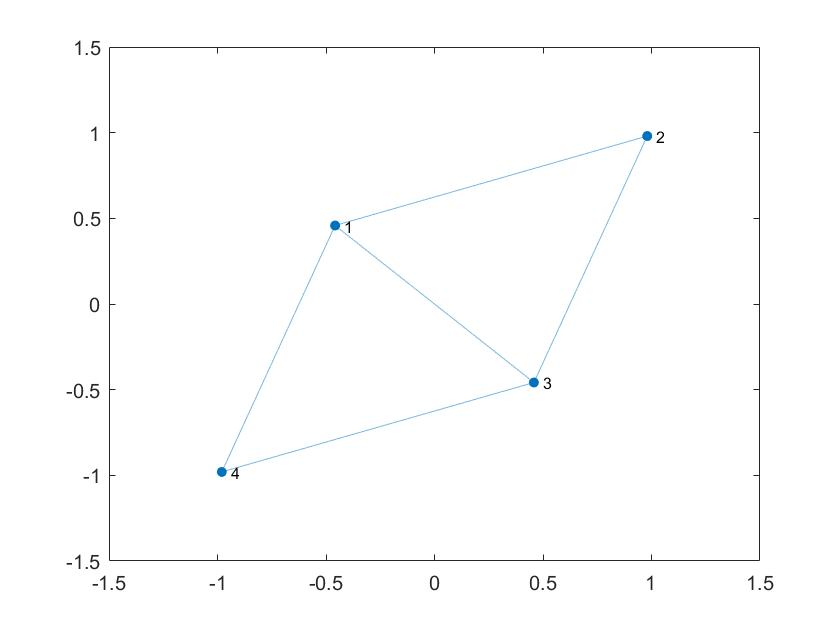
\includegraphics[width=340pt,height=270pt]{figure1.jpg}
    \caption{示例无向图}
\end{figure}
\begin{center}
    \begin{lstlisting}[caption={FirstExample.m},language=Matlab]
        %This is example1.m
A = [0, 1, 1, 1; ...
    1, 0, 1, 0; ...
    1, 1, 0, 1; ...
    1, 0, 1, 0;];
G = graph(A);
plot(G);
        %This is example2.m
s = [1, 2, 3, 3, 4];
t = [2, 3, 4, 1, 1];
G = graph(s, t);
plot(G);
        %This is example3.m
s = [1, 2, 3, 3, 4];
t = [2, 3, 4, 1, 1];
w = [9, 8, 7, 5, 2];
G = graph(s, t, w);
plot(G, 'EdgeLabel', G.Edges.Weight, 'linewidth', 2);  
%Please read Mathwork graph-plot for more information.
        %This is example4.m
s = [1, 2, 3, 3, 4];
t = [2, 3, 4, 1, 1];
w = [9, 8, 7, 5, 2];
nodesname = {'Alpha', 'Beta', 'Gamma', 'Delta'};
G = graph(s, t, w, nodesname);
plot(G, 'EdgeLabel', G.Edges.Weight, 'linewidth', 2); 
set(gca, 'XTick', [], 'YTick', []);

        \end{lstlisting}
\end{center}


\subsubsection{树的基本概念}
\par 6.树,一个树类似于一个连通的无向图。
\\当且仅当一幅含有V个结点的图G满足下列五个条件之一时,它就是一棵树:
\\G有V-1条边且不含有环
\\G有V-1条边且是连通的
\\G是连通的,但删除任意一条边都会使它不再连通
\\G是无环图,但添加任意一条边都会产生一条环
\\G中的任意一对顶点之间仅存在一条简单路径。
\\树的定义有些许抽象,我们来点实际例子。

\par \noindent 连线问题的数学模型是在连通赋权图上求权最小的生成树。赋权图的具最小权的生
成树叫做最小生成树。
主要有prim 算法构造最小生成树与 Kruskal 算法构造最小生成树。同时还可以用这两个算法求解。
\subsubsection{Matlab实现-matlab生成树}
\fbox{
    \parbox{\textwidth}{
        matlab生成树提供的函数有:
        \\  返回图G生成的最小生成树,(Name与Value用来枝定生成算法)
        \\  T = minspantree(G,Name,Value);
        \\  从一个源节点到另一个节点的最短路径树
        \\  TR = shortestpathtree(G,s,t,Name,Value);
        \\

    }
}
\begin{figure}[h]
    \centering
    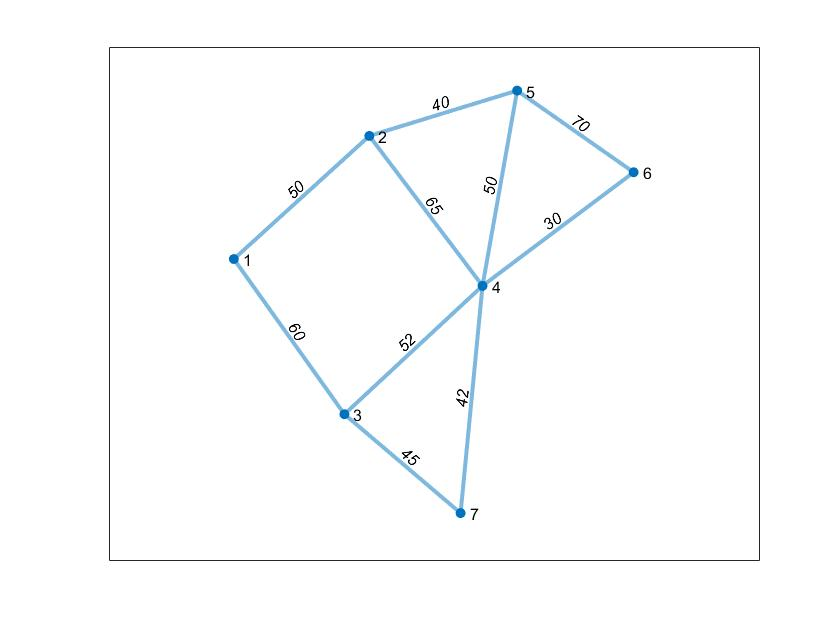
\includegraphics[width=340pt,height=270pt]{figure2.jpg}
    \caption{示例生成树}
\end{figure}
\begin{center}
    \begin{lstlisting}[caption={SecondExample.m},language=Matlab]
        %This is example1.m
A = [0, 1, 1, 0, 0, 0, 0; ...
    1, 0, 0, 1, 1, 0, 0; ...
    1, 0, 0, 1, 0, 0, 1; ...
    0, 1, 1, 0, 1, 1, 1; ...
    0, 1, 0, 1, 0, 1, 0; ...
    0, 0, 0, 1, 1, 0, 0; ...
    0, 0, 1, 1, 0, 0, 0];
G = graph(A);
G.Edges.Weight(1) = 50;
G.Edges.Weight(2) = 60;
G.Edges.Weight(3) = 65;
G.Edges.Weight(4) = 40;
G.Edges.Weight(5) = 52;
G.Edges.Weight(6) = 45;
G.Edges.Weight(7) = 50;
G.Edges.Weight(8) = 42;
G.Edges.Weight(8) = 30;
G.Edges.Weight(9) = 42;
G.Edges.Weight(10) = 70;
plot(G, 'EdgeLabel', G.Edges.Weight, 'linewidth', 2)
        %This is example2.m
clc;
clear;
a = zeros(7);
a(1, 2) = 50;a(1, 3) = 60;
a(2, 4) = 65;a(2, 5) = 40;
a(3, 4) = 52;a(3, 7) = 45;
a(4, 5) = 50;a(4, 6) = 30;a(4, 7) = 42;
a(5, 6) = 70;
a = a + a';
a(find(a == 0)) = inf;
result = [];
p = 1;
tb = 2:length(a);
while length(result) ~= length(a) - 1
    temp = a(p, tb);
    temp = temp(:);
    d = min(temp);
    [jb, kb] = find(a(p, tb) == d);
    j = p(jb(1));
    k = tb(kb(1));
    result = [result, [j; k; d]];
    p = [p, k];
    tb(find(tb == k)) = [];
end
result
        %This is example3.m
clc;
clear;
a(1, 2) = 50;a(1, 3) = 60;
a(2, 4) = 65;a(2, 5) = 40;
a(3, 4) = 52;a(3, 7) = 45;
a(4, 5) = 50;a(4, 6) = 30;a(4, 7) = 42;
a(5, 6) = 70;
[i, j, b] = find(a);
data = [i'; j'; b'];
index = data(1:2, :);
loop = max(size(a)) - 1;
result = [];
while length(result) < loop
    temp = min(data(3, :));
    flag = find(data(3, :) == temp);
    flag = flag(1);
    v1 = data(1, flag);
    v2 = data(2, flag);
    if index(1, flag) ~= index(2, flag)
        result = [result, data(:, flag)];
    end
    index(find(index == v2)) = v1;
    data(:, flag) = [];
    index(:, flag) = [];
end
s = result(1, :);
t = result(2, :);
w = result(3, :);
G = graph(s, t, w);
plot(G, 'EdgeLabel', G.Edges.Weight, 'linewidth', 2);
result
        \end{lstlisting}
\end{center}
\subsection{图与网络示例}
\fbox{
    \parbox{\textwidth}{
        例子1.求图3.中$v_1$到$v_{11}$的最短路径。可以使用graphshortestpath函数来寻找最短的距离,并且给出
        沿着这个最短路径的各个节点。
    }
}
\begin{figure}[H]
    {
        \centering
        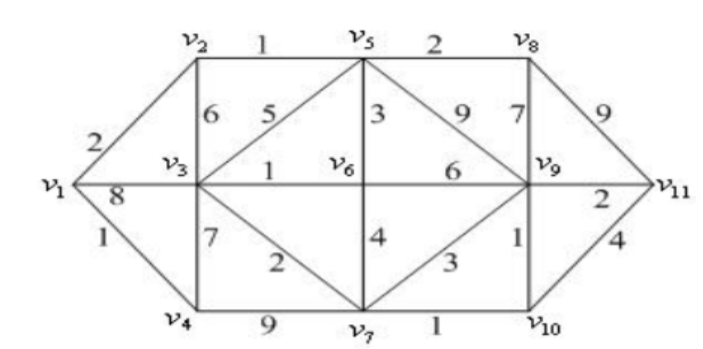
\includegraphics[width=0.8\textwidth]{figure2.png}
        \caption{无向图的最短路径}
    }
\end{figure}
\begin{center}
    \begin{lstlisting}[caption={Example1.m},language=Matlab]
        %This is example1.m
        clc,clear;
        a(1,2)=2;a(1,3)=8;a(1,4)=1;
        a(2,3)=6;a(2,5)=1;
        a(3,4)=7;a(3,5)=5;a(3,6)=1;a(3,7)=2;
        a(4,7)=9;
        a(5,6)=3;a(5,8)=2;a(5,9)=9;
        a(6,7)=4;a(6,9)=6;
        a(7,9)=3;a(7,10)=1;
        a(8,9)=7;a(8,11)=9;
        a(9,10)=1;
        a(9,11)=2;
        a(10,11)=4;
        a=a';
        [i,j,v]=find(a);
        b = sparse(i,j,v,11,11);
        [x,y,z]=graphshortestpath(b,1,11,'Directed',false);
        disp('The shortest distance = ');
        disp(x);%  13
        disp('The path =');
        disp(y);
        %  1     2     5     6     3     7    10     9    11
        \end{lstlisting}
\end{center}
\fbox{
    \parbox{\textwidth}{
        例子2.求图4.有向图$v_s$到$v_t$的最短路径及长度。
    }
}
\begin{figure}[h]
    \begin{center}
        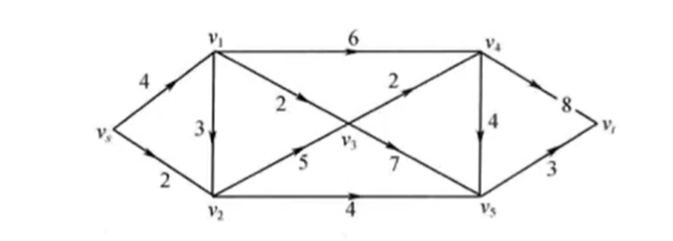
\includegraphics[width=0.80\textwidth]{figure3.png}
        \caption{有向图的最短路径}
    \end{center}
\end{figure}
\begin{center}
    \begin{lstlisting}[caption={Example2.m},language=Matlab]
        %This is example2.m
clc,clear;
a=zeros(7);
a(1,2)=4;a(1,3)=2;
a(2,3)=3;a(2,4)=2;a(2,5)=6;
a(3,4)=5;a(3,6)=4;
a(4,5)=2;a(4,6)=7;
a(5,6)=4;a(5,7)=8;
a(6,7)=3;
b=sparse(a);
[x,y,z]=graphshortestpath(b,1,7,'Directed',1,'Method','Bellman-Ford');
view(biograph(b,[]));
        \end{lstlisting}
\end{center}

\par \fbox{
    \parbox{\textwidth}{
        例子3.如下表,设有九个节点$v_i(i=1,2,\cdots,9)$,坐标分别为$(x_i,y_i)$,具体数据见下表。任意两个节点之间的距离为
        $$ d_{ij}=|x_i-x_j|+|y_i-y_j|$$。
        问怎样连接电缆,使每个节点都连通,且所用的总电缆长度为最短?
    }
}
\begin{center}
    \begin{table}[h]
        \centering
        \caption{点的数据坐标}
        \begin{tabular}{c|c|c|c|c|c|c|c|c|c}
            \hline
            i     & 1  & 2  & 3  & 4  & 5  & 6  & 7  & 8  & 9  \\
            \hline
            $x_i$ & 0  & 5  & 16 & 20 & 33 & 23 & 35 & 25 & 10 \\
            \hline
            $y_i$ & 15 & 20 & 24 & 20 & 25 & 11 & 7  & 0  & 3  \\
            \hline
        \end{tabular}
    \end{table}
\end{center}
\begin{center}
    \begin{lstlisting}[caption={Example3.m},language=Matlab]
        %This is example3.m
clc,clear;
x=[0,5,16,20,33,23,35,25,10];
y=[15,20,24,20,25,11,7,0,3];
xy=[x;y];
d=mandist(xy);
d=tril(d);
b=sparse(d)
[ST,pred]=graphminspantree(b,'Method','Kruskal');
st=full(ST);
TreeLength=sum(sum(st))
view(biograph(ST,[],'ShowArrows','off'));
        \end{lstlisting}
\end{center}
\par \fbox{
    \parbox{\textwidth}{
        例子4.求下图中从\ding{172}到\ding{179}的最大流。
    }
}
\begin{figure}[h]
    \begin{center}
        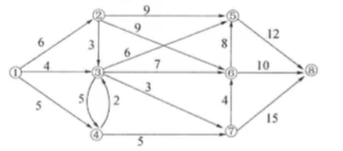
\includegraphics[width=0.8\textwidth]{figure4.png}
        \caption{最大流问题的网络图}
    \end{center}
\end{figure}
\begin{center}
    \begin{lstlisting}[caption={Example4.m},language=Matlab]
        %This is example4.m
clc,clear;
a=zeros(9);
a(1,2)=6;a(1,3)=4;a(1,4)=5;
a(2,3)=3;a(2,5)=9;a(2,6)=9;
a(3,4)=4;a(3,5)=6;a(3,6)=7;a(3,7)=3;
a(4,7)=5;a(4,9)=2;
a(5,8)=12;
a(6,5)=8;a(6,8)=10;
a(7,6)=4;a(7,8)=15;
a(9,3)=2;
b=sparse(a);
[x,y,z]=graphmaxflow(b,1,8)
        \end{lstlisting}
\end{center}
\section{图与网络-代码实现}
\par 贴出matlab代码求解,请结合前面整理后的式子来分别对应变量
\begin{center}
    \begin{lstlisting}[caption={Picture and Network},language=Matlab]
clc,clear
a=zeros(6);
a(1,2)=50;a(1,4)=40;a(1,5)=25;a(1,6)=10;
a(2,3)=15;a(2,4)=20;a(2,6)=25;
a(3,4)=10;a(3,5)=20;
a(4,5)=10;a(4,6)=25;
a(5,6)=55;
a=a+a';
a(find(a==0))=inf;
pb(1:length(a))=0;pb(1)=1;index1=1;index2=ones(1,length(a));
d(1:length(a))=inf;d(1)=0;temp=1;
while sum(pb)<length(a)
 tb=find(pb==0);
 d(tb)=min(d(tb),d(temp)+a(temp,tb));
 tmpb=find(d(tb)==min(d(tb)));
 temp=tb(tmpb(1));
 pb(temp)=1;
 index1=[index1,temp];
 temp2=find(d(index1)==d(temp)-a(temp,index1));
 index2(temp)=index1(temp2(1));
end
d, index1, index2
        \end{lstlisting}
\end{center}

\section{图与网络-实战演练}
\par 国赛很需要图与网络去做一些特殊解法,同时图与网络也是其他算法所必须要学习的东西,推荐进行学习。做题的话可以看
\newpage
\begin{thebibliography}{99}
    \bibitem{ref1}谢中华. MATLAB与数学建模[A].北京航空航天大学出版社[M]:科学技术协会,2021-02-14.
    \bibitem{ref2}数学建模老师. 第9讲 图与网络模型及方法(一)[M]:\url{https://www.bilibili.com/video/BV1na411Y7kP/?spm_id_from=333.337.search-card.all.click&vd_source=1db675367482476693cd8659d026e5b7},2022-04-25.
    \bibitem{ref3}英雄哪里出来. 算法学习路线[A].\url{https://ufbva3m5zn.feishu.cn/docs/doccnIQ95UPr5yabjQg2bFHl79f},2023-7-23.
    \bibitem{ref4}letterMe.第二章--网络与图(复杂网络学习笔记)[A].\url{https://www.cnblogs.com/GGTomato/p/12654337.html}, 2020-04-07 .
    \bibitem{ref5}Miao\_Guo.图的一些基本知识:图,邻居,度矩阵,邻接矩阵[B].\url{https://blog.csdn.net/luzaijiaoxia0618/article/details/104718146},2020-03-07.
    \bibitem{ref6}Miao\_Guo.图的一些基本知识:关联矩阵、拉普拉斯矩阵[B].\url{https://blog.csdn.net/luzaijiaoxia0618/article/details/104720948},2020-03-08.
    \bibitem{ref7}HachiLin.图论基础知识(二) —— 路与连通[B]\url{https://blog.csdn.net/Hachi_Lin/article/details/88047555}, 2019-02-28.
    \bibitem{ref8}Mathwork.(graph)具有无向边的图[M].\url{https://ww2.mathworks.cn/help/matlab/ref/graph.html},
    \bibitem{ref9}Mathwork.(digraph)具备有向边的图[M].\url{https://ww2.mathworks.cn/help/matlab/ref/digraph.html},
    \bibitem{ref10}Better-ing.matlab 绘制有向图、无向图、有权有向图、有权无向图以及查找最短路径[B].\url{https://blog.csdn.net/weixin_43404836/article/details/114252343},2021-03-01.
    %\bibitem{ref10}Better-ing.matlab 绘制有向图、无向图、有权有向图、有权无向图以及查找最短路径[B].\url{https://blog.csdn.net/weixin_43404836/article/details/114252343?spm=1001.2101.3001.6650.9&utm_medium=distribute.pc_relevant.none-task-blog-2%7Edefault%7EBlogCommendFromBaidu%7ERate-9-114252343-blog-125569212.235%5Ev38%5Epc_relevant_anti_vip_base&depth_1-utm_source=distribute.pc_relevant.none-task-blog-2%7Edefault%7EBlogCommendFromBaidu%7ERate-9-114252343-blog-125569212.235%5Ev38%5Epc_relevant_anti_vip_base&utm_relevant_index=15},2021-03-01.
    \bibitem{ref11}Mathwork.GraphPlot 属性-图论图的外观和行为[M].\url{https://ww2.mathworks.cn/help/matlab/ref/matlab.graphics.chart.primitive.graphplot-properties.html},
    \bibitem{ref12} MARK\_REAPER.Matlab图论工具箱的利用[B].\url{https://www.cnblogs.com/markReaper/p/8454817.html},2018-02-20 .
\end{thebibliography}
\newpage
\section{数学建模算法大全第五章习题答案}
\begin{itemize}
    \item[1.]简单思考可知,先运羊,接着随意带狼(菜)到对岸,再把羊带回去,再把菜(狼)带对岸,最后带羊回去即可。
    \item[2.]简单可见图如下:
    \begin{figure}[h]
        \begin{center}
            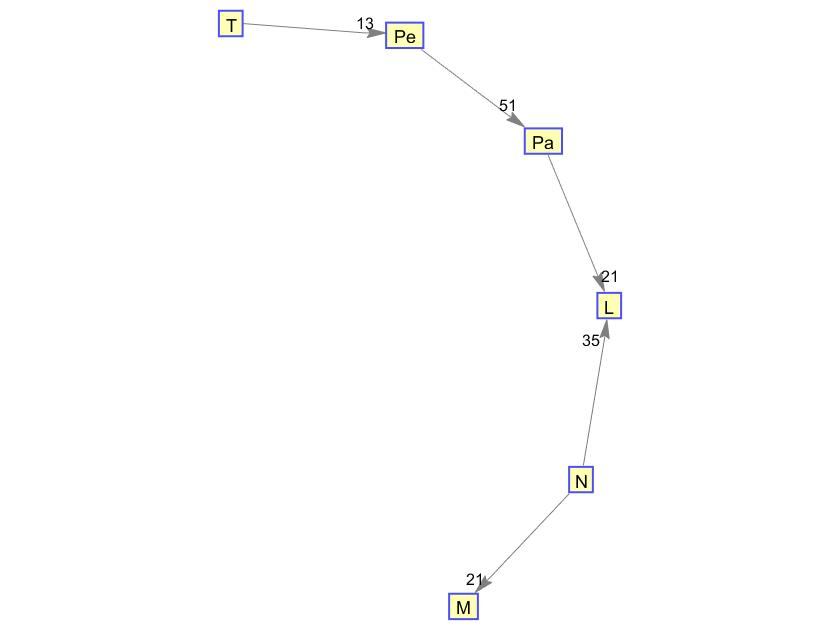
\includegraphics[width=0.8\textwidth]{figure3.jpg}
        \end{center}
    \end{figure}
    \item[3.] 第二年处和第三年初都换一台新机器,总费用4万元。
    \item[4.] 从仓库运往市场的最大流量为110单位,其中市场3只能满足50单位,差10单位。
    \item[5.] 甲未得到聘用,乙-俄,丙-日,丁-英,戊-德。
    \item[6.] 最小费用为240。
\end{itemize}

\end{document}